\newpage
\tikz[remember picture,overlay] \node[opacity=1,inner sep=0pt] at (current page.center){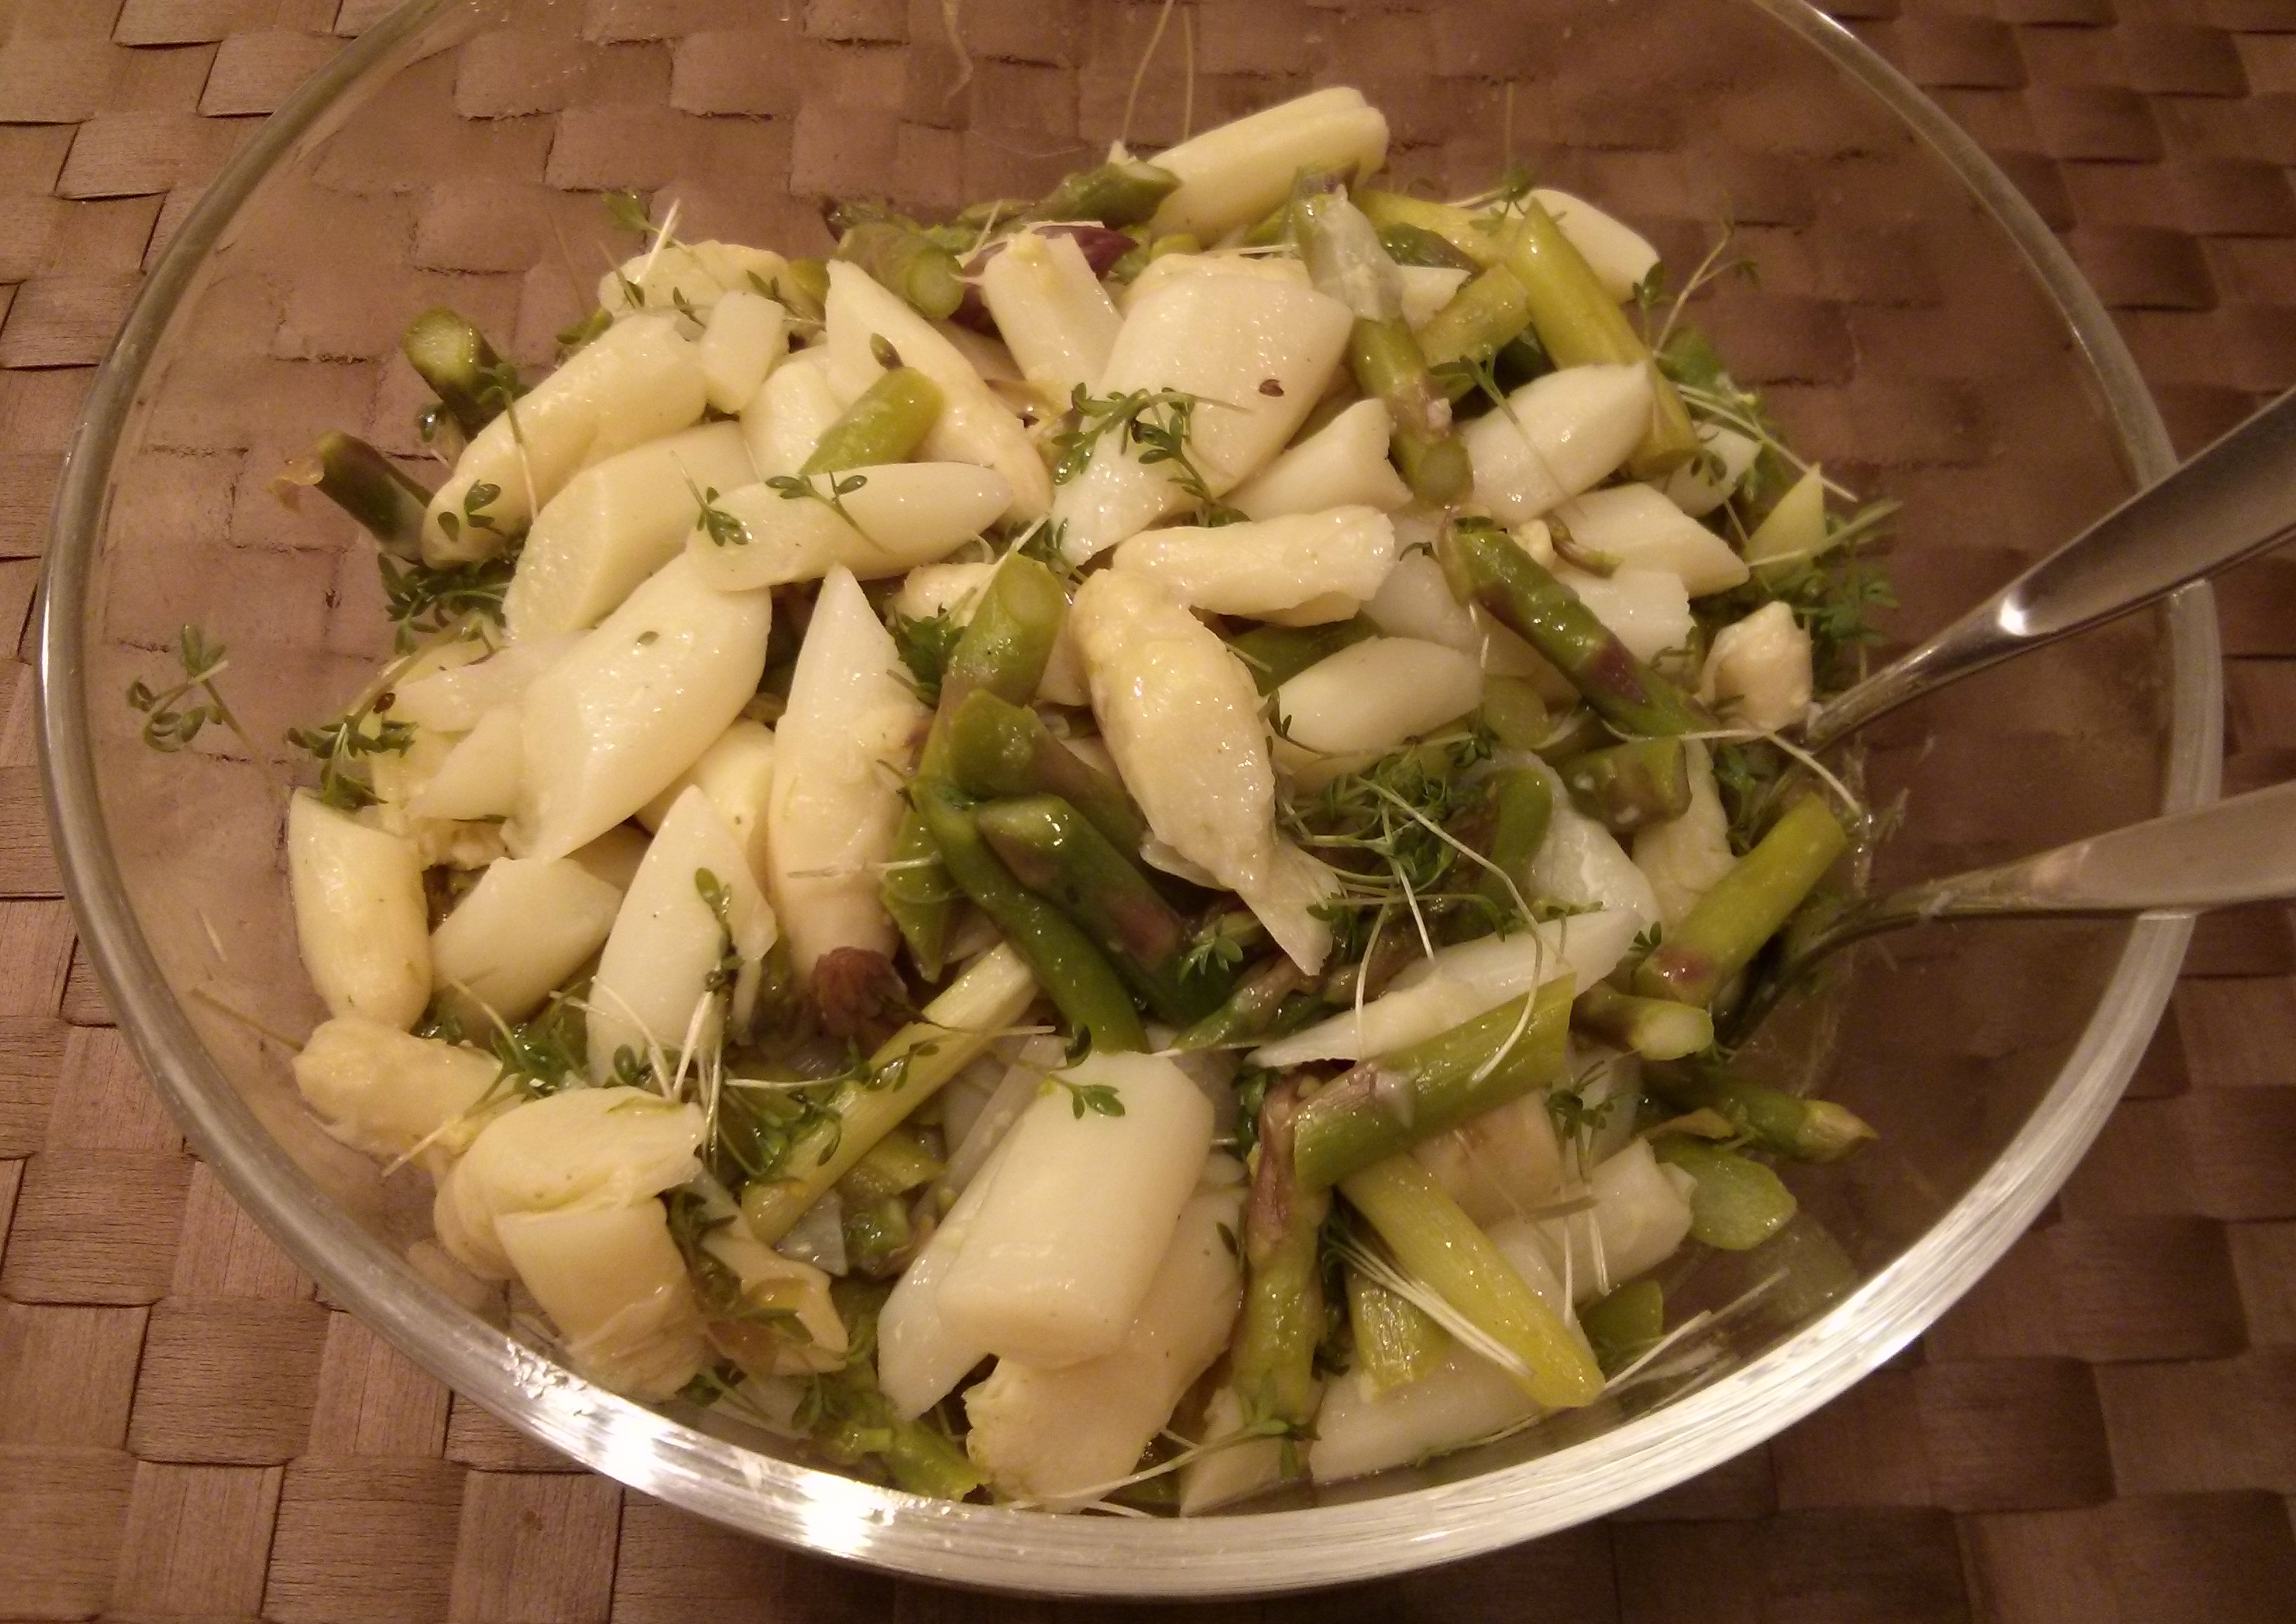
\includegraphics[width=\paperwidth,height=\paperheight]{./bilder/spargelsalat_ratio.jpg}};

\begin{recipe}[]{Warmer Spargelsalat} %Quelle
	\timerecipe[Minuten]{ca. 30} %mit [EINHEIT]
	\personcount{2} % mit[ART]
	\ingredient{500g Spargel (weiß/grün/gemischt)} % ggf. \nicefrac{1}{2}
	\ingredient{Traubenkernöl}
	\ingredient{weißer Balsamico}
	\ingredient{Brunnenkresse}
	\ingredient{Salz}
	\ingredient{Pfeffer}
	\ingredient{Zucker}
	\ingredient{Zitronensaft}


\step
\textbf{Spargel} schälen (grünen Spargel nur im unteren Drittel) und in 3-4cm lange Stückchen schneiden.

\step
Spargel mit etwas \textbf{Salz}, \textbf{Zucker}, \textbf{Butter} und \textbf{Zitronensaft} im Wasser kochen (grüner Spargel ist schneller gar als weißer, als erst später ins Wasser geben).

\step
Während der Spargel etwas abkühlt aus \textbf{Traubenkernöl}, \textbf{weißem Balsamico}, \textbf{Salz} und \textbf{Pfeffer} eine Salatsoße mischen.

\step
Spargel vorsichtig mit der Salatsoße mischen und die \textbf{Brunnenkresse} darauf drapieren. Lauwarm servieren.

%\tippbox{\textbf{Tipp:} ...} % Tipp in extra Rahmen
\end{recipe}